\documentclass[main.tex]{subfiles}
\begin{document}
\newpage
	\section{Introduction}
	This document describes how to install and run the different parts of our system.\\
	In figure \ref{fig:architecture} you can see the architecture of our system.
	\begin{figure}[h]
\centering
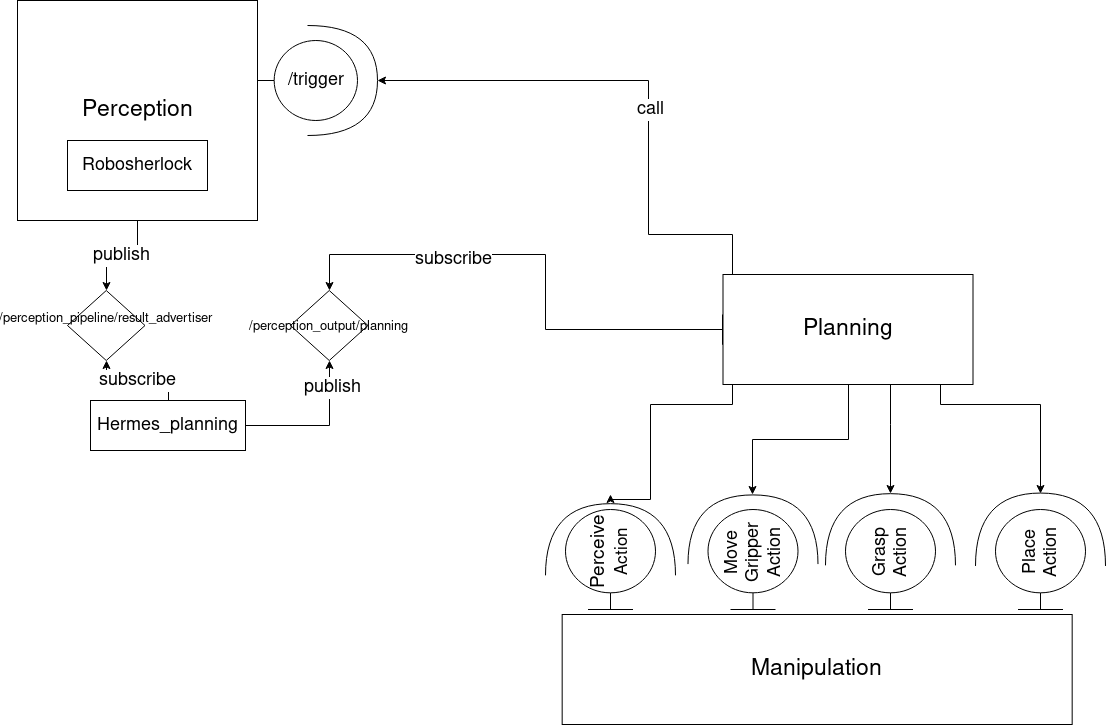
\includegraphics[width=0.8\textwidth]{architecture/architecture}
\caption{Architecture}
\label{fig:architecture}
\end{figure}
	
	\subsection{Prerequisites}
	
	Because of different dependencies our system only runs on \textbf{Ubuntu 16.04 64-bit}.\\
	To install dependencies we use pip. Run the following commands to install pip:
	\begin{lstlisting}
sudo apt install python-pip
sudo apt install python3-venv python3-pip
\end{lstlisting}
Because sometimes problems with different python-scipy versions occure, we recommend to run:
\begin{lstlisting}
sudo pip install scipy==1.2.2
\end{lstlisting}
	The system runs with ROS-Kinetic. Instructions on how to install ROS can be found \href{http://wiki.ros.org/kinetic/Installation/Ubuntu}{here}. We recommend to install the Desktop-Full version.\\
	Since we work with the HSR you have to setup your PC for that.
	A description on how to do that can be found \href{https://docs.hsr.io/manual_en/howto/pc_install.html}{here}.\\
	We furthermore use some tools for the installation. These need to be installed before you install our system.\\
	The first tool you need is the catkin\_tools package. You find the instructions on how to install it \href{https://catkin-tools.readthedocs.io/en/latest/installing.html}{here}.\\
	We also use python-wstool.
	You can install it by running this command:
	\begin{lstlisting}
sudo apt-get install python-rosinstall python-wstool
\end{lstlisting}

If you had ROS already installed, it is advised to run:
\begin{lstlisting}
rosdep update
\end{lstlisting}
The "\textbackslash" at the end of the first line in the commands, that go over two lines, is needed if you copy the commands into your terminal. If you write the commands manually they are not needed.
	
	\subsection{Workspaces}
	\subsubsection{Create a Workspace}
	The first step is to open the directory where you want to create the workspace.\\
	Now run the following commands.
	\begin{lstlisting}
source /opt/ros/kinetic/setup.bash
mkdir -p YOURWORKSPACENAME/src
cd YOURWORKSPACENAME/
catkin build 
\end{lstlisting}
	
	To load the environment of a workspace, you can run the command:
	\begin{lstlisting}
source devel/setup.bash
\end{lstlisting}
	in your workspace.
	
	\subsubsection{How we manage our Workspaces} \label{workspace_management}
	
	We use three workspaces for our system, since using just one causes some problems.\\
	The first workspace contains the \nameref{sec:Manipulation} part (without Navigation).\\
	In the second workspace we installed the \nameref{sec:Planning} part.\\
	Everything else can be installed in the third workspace.\\
	To create the workspaces we use, run:\\
	\begin{lstlisting}
source /opt/ros/kinetic/setup.bash
mkdir -p manipulation_ws/src
cd manipulation_ws/
catkin build 
cd ..
mkdir -p planning_ws/src
cd planning_ws/
catkin build 
cd ..
mkdir -p suturo_ws/src
cd suturo_ws/
catkin build 
\end{lstlisting}
	
	We dont source our workspaces in the .bashrc. Instead we run\\
	\begin{lstlisting}
source devel/setup.bash
\end{lstlisting}
to source the relevant workspace in our terminal, before starting a part of our system.
	

\end{document}
